\documentclass[11pt]{article}

\usepackage[margin=1in]{geometry}
\usepackage{amsmath, amssymb}
\usepackage{graphicx}
\usepackage{booktabs}
\usepackage{enumitem}
\usepackage{xcolor}
\usepackage[colorlinks=true, linkcolor=blue, citecolor=blue, urlcolor=blue]{hyperref}

\newcommand{\ket}[1]{\left|#1\right\rangle}
\newcommand{\bra}[1]{\left\langle#1\right|}
\newcommand{\RZZ}{R_{ZZ}}
\newcommand{\RZX}{R_{ZX}}

% Figures are generated by make_state_transfer_circuits.py in this folder.
\graphicspath{{./}}

\title{Cross-Chip Gates by Coherent State Transfer Only:\\
Ping-Pong vs.\ Migration (No Mid-Circuit Measurement)}
\author{Companion to \texttt{locc\_ejpp\_tutorial.tex}; figures from
\texttt{make\_state\_transfer\_circuits.py}}
\date{July 2026}

\begin{document}
\maketitle

\begin{abstract}
The EJPP telegate implements a cross-chip gate with one ebit and two
mid-circuit measurements. This note works out the fully \emph{coherent}
alternative: use the cable's quantum state transfer (QST) as a unitary
``move'' operation and do every two-qubit gate locally. No measurement, no
feedforward, no classical bits, no Pauli frame. We give the transfer
operator, prove the two implementation patterns (\emph{ping-pong}: two cable
traversals per gate; \emph{migration}: two traversals \emph{total}), show
the exact algebraic condition that decides which one a circuit admits, and
apply both to \texttt{HF\_8q\_3doubles\_rzx.json}. All circuits shown here
were verified unitarily equivalent to their nonlocal targets by the
companion script.
\end{abstract}

\section{The transfer operator}

From \texttt{qst\_formulas.txt}, the cable executes a full state transfer in
$\tau \approx 66$~ns:
\[
\big(\alpha\ket{0} + \beta\ket{1}\big)_{\!A}\,\ket{0}_R\,\ket{0}_B
\;\longrightarrow\;
\ket{0}_A\,\ket{0}_R\,\big(\alpha\ket{0} + \beta\ket{1}\big)_{\!B},
\]
i.e.\ on the (sender, receiver) pair, with the receiver guaranteed to start
in $\ket{0}$, it acts as a SWAP. We write $T$ for the transfer
sender$\to$receiver and note two properties used throughout:

\begin{enumerate}[leftmargin=2em]
  \item \textbf{Self-cleaning $\ket{0}$ bookkeeping.} $T$ leaves the sender
        in $\ket{0}$ --- which is exactly the empty receiver that the return
        transfer $T^{\dagger}$ requires. The ``hole'' shuttles back and
        forth inside the communication pair and never touches data.
  \item \textbf{Disjoint support $\Rightarrow$ commutation.} $T$ acts only on
        the travelling qubit, the cable mode, and the ancilla. For any gate
        $V$ on \emph{other} qubits,
        \[
        T\,V\,T^{\dagger} = V
        \qquad\text{(equivalently } TV = VT\text{).}
        \]
\end{enumerate}

\section{Toy model}

Four qubits. Chip A holds data qubits $A_0, A_1$ ($A_1$ is the seam qubit
that will travel); chip B holds data qubit $B_0$ and a communication ancilla
$e$ initialized to $\ket{0}$. The target circuit is three cross-chip gates
with local layers in between:
\begin{equation}
U \;=\; R_3\, V_2\, R_2\, V_1\, R_1,
\qquad
R_k = \RZZ(t_k)\ \text{on}\ (A_1, B_0),
\label{eq:target}
\end{equation}
with $V_1 = H_{A_0} \otimes R_Z(\varphi)_{A_1}$ and
$V_2 = H_{A_0} \otimes Z_{B_0}$. Note $V_1$ touches the travelling qubit
$A_1$, but only with a \emph{single-qubit} gate --- this matters below.

\begin{figure}[h]
\centering
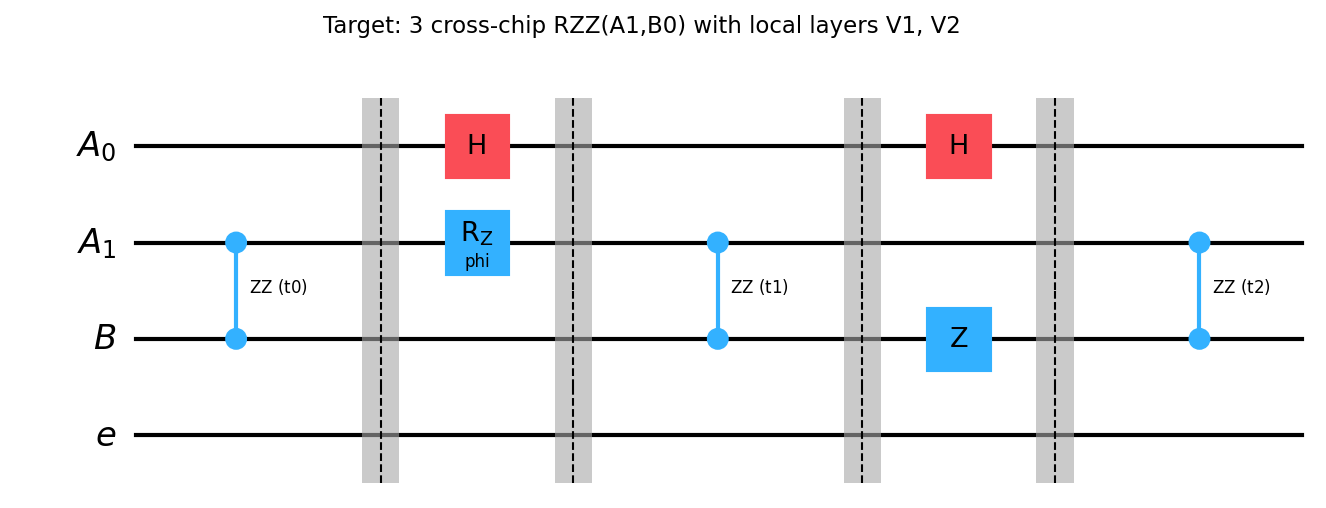
\includegraphics[width=0.9\textwidth]{fig1_toy_target.png}
\caption{The nonlocal target~\eqref{eq:target}: three $\RZZ(t_k)$ straddle
the chip cut (between $A_1$ and $B_0$); the ancilla $e$ is idle. This is the
circuit we must reproduce without any gate crossing the cut.}
\label{fig:target}
\end{figure}

\subsection{Ping-pong: two traversals per gate}

The basic identity: a nonlocal $\RZZ$ equals transfer out, local gate
against the ancilla, transfer back,
\begin{equation}
\RZZ(\theta)_{A_1 B_0} \;=\; T^{\dagger}\, \RZZ(\theta)_{e B_0}\, T .
\label{eq:sandwich}
\end{equation}
Proof on a basis state: $T$ carries the bit value $x$ of $A_1$ onto $e$; the
local gate imprints $e^{-i\frac{\theta}{2}(-1)^{x\oplus y}}$, exactly the
phase the nonlocal gate would have imprinted; $T^{\dagger}$ returns $x$ to
$A_1$. Substituting \eqref{eq:sandwich} for each $R_k$
in~\eqref{eq:target}:
\begin{equation}
U \;=\;
\big(T^{\dagger} L_3 T\big)\, V_2\,
\big(T^{\dagger} L_2 T\big)\, V_1\,
\big(T^{\dagger} L_1 T\big),
\qquad L_k \equiv \RZZ(t_k)_{e B_0}.
\label{eq:pingpong}
\end{equation}
Six $T$'s appear: \textbf{six cable traversals, with the data on the wire
every time} (Fig.~\ref{fig:pingpong}). Everything is unitary and
deterministic --- already no measurement is needed.

\begin{figure}[h]
\centering
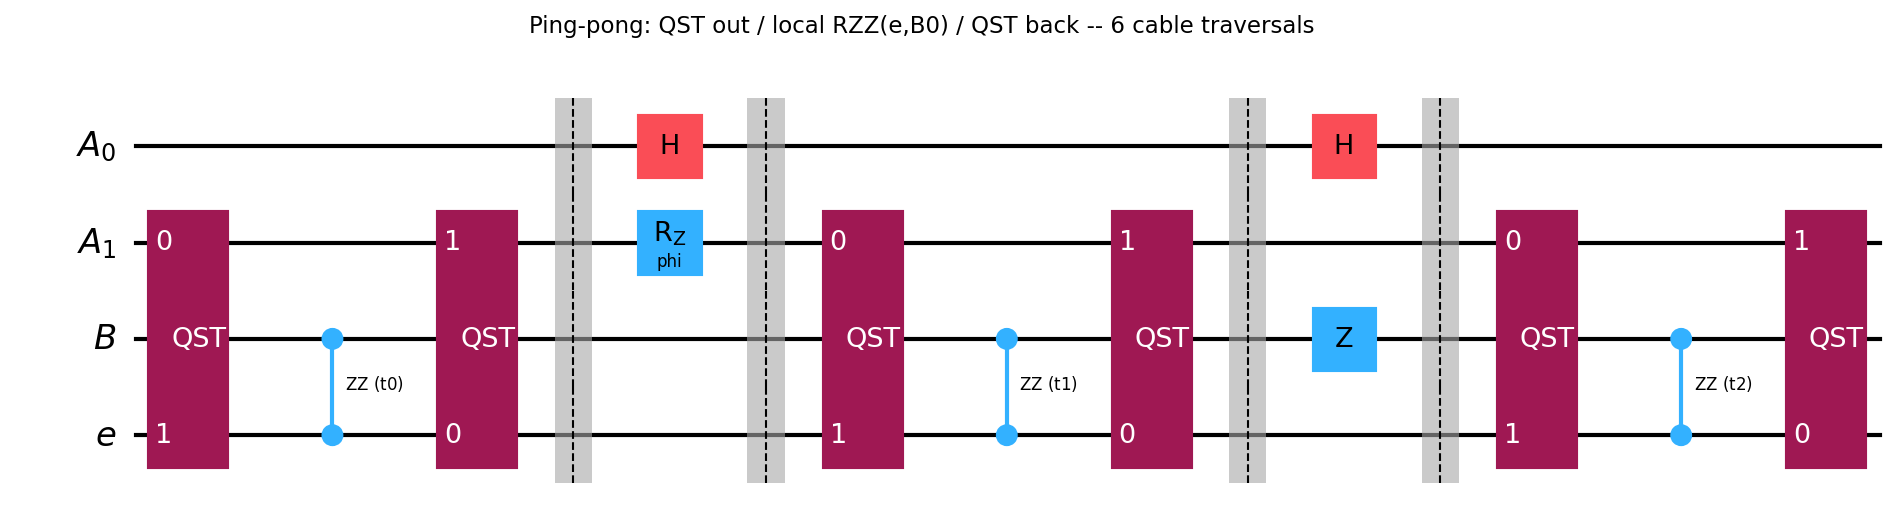
\includegraphics[width=\textwidth]{fig2_toy_pingpong.png}
\caption{Ping-pong implementation of Fig.~\ref{fig:target}. Each QST box is
one cable traversal (drawn as the exact SWAP it enacts on the required
subspace). Every $\RZZ$ is now local on chip B; cost: 6 traversals.}
\label{fig:pingpong}
\end{figure}

\subsection{Migration: two traversals total}

If every intermediate layer commutes with $T$, the inner transfers cancel.
Slide each $V_i$ through the neighbouring transfers in~\eqref{eq:pingpong}
using $T V_i T^{\dagger} = V_i$:
\begin{equation}
U \;=\;
T^{\dagger} L_3 \underbrace{\big(T V_2 T^{\dagger}\big)}_{=\,V_2}
L_2 \underbrace{\big(T V_1 T^{\dagger}\big)}_{=\,V_1'} L_1\, T
\;=\;
T^{\dagger}\, \big(L_3 V_2 L_2 V_1' L_1\big)\, T .
\label{eq:telescope}
\end{equation}
All adjacent $T^{\dagger}T$ pairs annihilate. Read right to left: transfer
out \emph{once}, run the entire dressed sequence with the state living on
chip B, transfer home \emph{once} (Fig.~\ref{fig:migration}).

Two remarks on the condition:
\begin{itemize}[leftmargin=2em]
  \item \textbf{Single-qubit gates on the traveller are free.} $V_1$
        contains $R_Z(\varphi)$ on $A_1$; conjugation by $T$ just relabels
        it onto $e$: $V_1' = H_{A_0} \otimes R_Z(\varphi)_{e}$. The gate
        travels with the qubit and stays local.
  \item \textbf{Chip-B gates on the traveller are also free} --- they were
        the point of migrating.
\end{itemize}
The only forbidden pattern is stated in Section~\ref{sec:blocked}.

\begin{figure}[h]
\centering
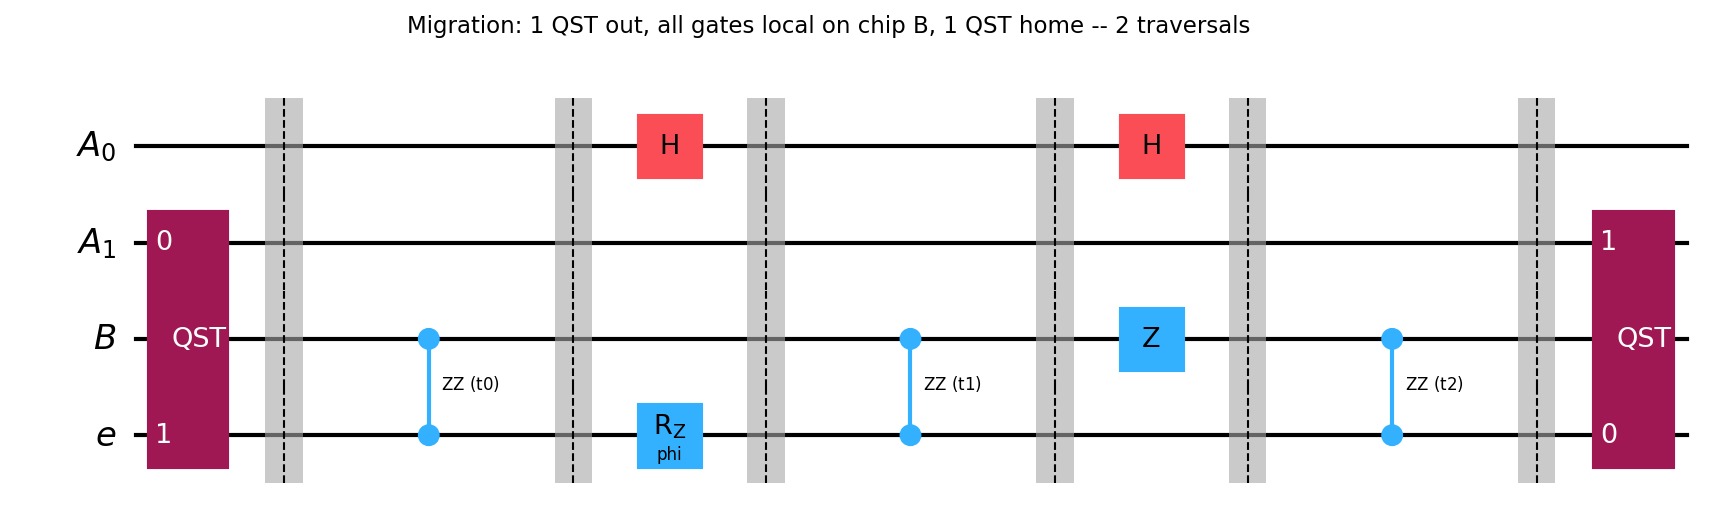
\includegraphics[width=\textwidth]{fig3_toy_migration.png}
\caption{Migration implementation of the same target: one QST out, all three
$\RZZ(t_k)$ and the $R_Z(\varphi)$ dressing local on chip B, one QST home.
Cost: 2 traversals. Verified unitarily identical to Fig.~\ref{fig:target}.}
\label{fig:migration}
\end{figure}

\subsection{When migration is blocked}
\label{sec:blocked}

Let $V_1 = \mathrm{CZ}(A_0, A_1)$: a two-qubit gate between the traveller
and a qubit that \emph{stayed on chip A}. Conjugation by $T$ relabels
$A_1 \to e$:
\[
T\, \mathrm{CZ}_{A_0 A_1}\, T^{\dagger} \;=\; \mathrm{CZ}_{A_0\, e},
\]
which spans the cut --- itself a cross-chip gate
(Fig.~\ref{fig:blocked}). The telescoping in~\eqref{eq:telescope} dies at
this layer: either bring the qubit home (back to ping-pong) or perform a
nonlocal CZ (the thing being avoided). Hence the rule:

\begin{center}
\fbox{\parbox{0.85\textwidth}{\textbf{Migration condition.} While the seam
qubit is abroad, it may receive any single-qubit gate and any two-qubit gate
with destination-chip qubits, but \emph{no two-qubit gate with a qubit of
its home chip}.}}
\end{center}

\begin{figure}[h]
\centering
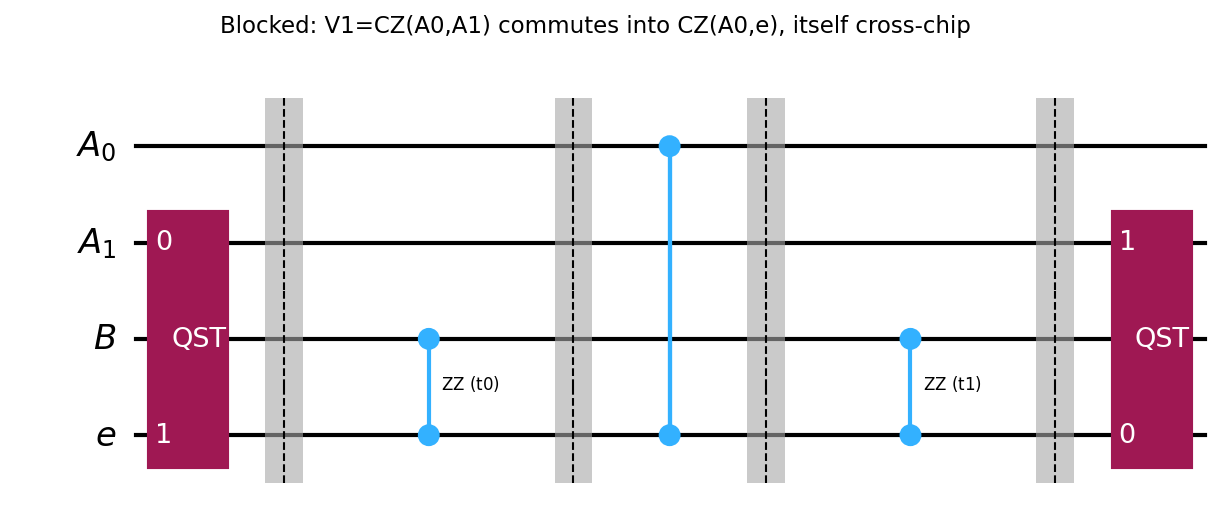
\includegraphics[width=0.85\textwidth]{fig4_toy_blocked.png}
\caption{The counterexample: with $V_1 = \mathrm{CZ}(A_0,A_1)$, migrating
$A_1$ turns the layer into $\mathrm{CZ}(A_0, e)$ --- the gate drawn here
between the top wire (chip A) and the bottom wire (chip B) crosses the cut,
so the 2-traversal scheme fails.}
\label{fig:blocked}
\end{figure}

\section{Application to \texttt{HF\_8q\_3doubles\_rzx}}

Chip A $= q_0\ldots q_3$, chip B $= q_4\ldots q_7$ plus one communication
ancilla $e$. The only cross-chip gates are the three $\RZX(t_k)$ on
$(q_6, q_2)$.

\subsection{What runs today: ping-pong (exact)}

Replace each $\RZX(t_k)_{q_6 q_2}$ by
$\;T_{q_2 \to e}\;\RZX(t_k)_{q_6 e}\;T_{e \to q_2}$.
Figure~\ref{fig:hfpp} shows the full 9-wire circuit; the companion script
verifies it equals the original 8-qubit unitary. Cost: 6 traversals, zero
measurements, total added seam time $\approx 6 \times 66\,\mathrm{ns}
\approx 0.4\,\mu s$ (plus local routing), negligible against
$T_1 = 85\,\mu s$.

\begin{figure}[h]
\centering
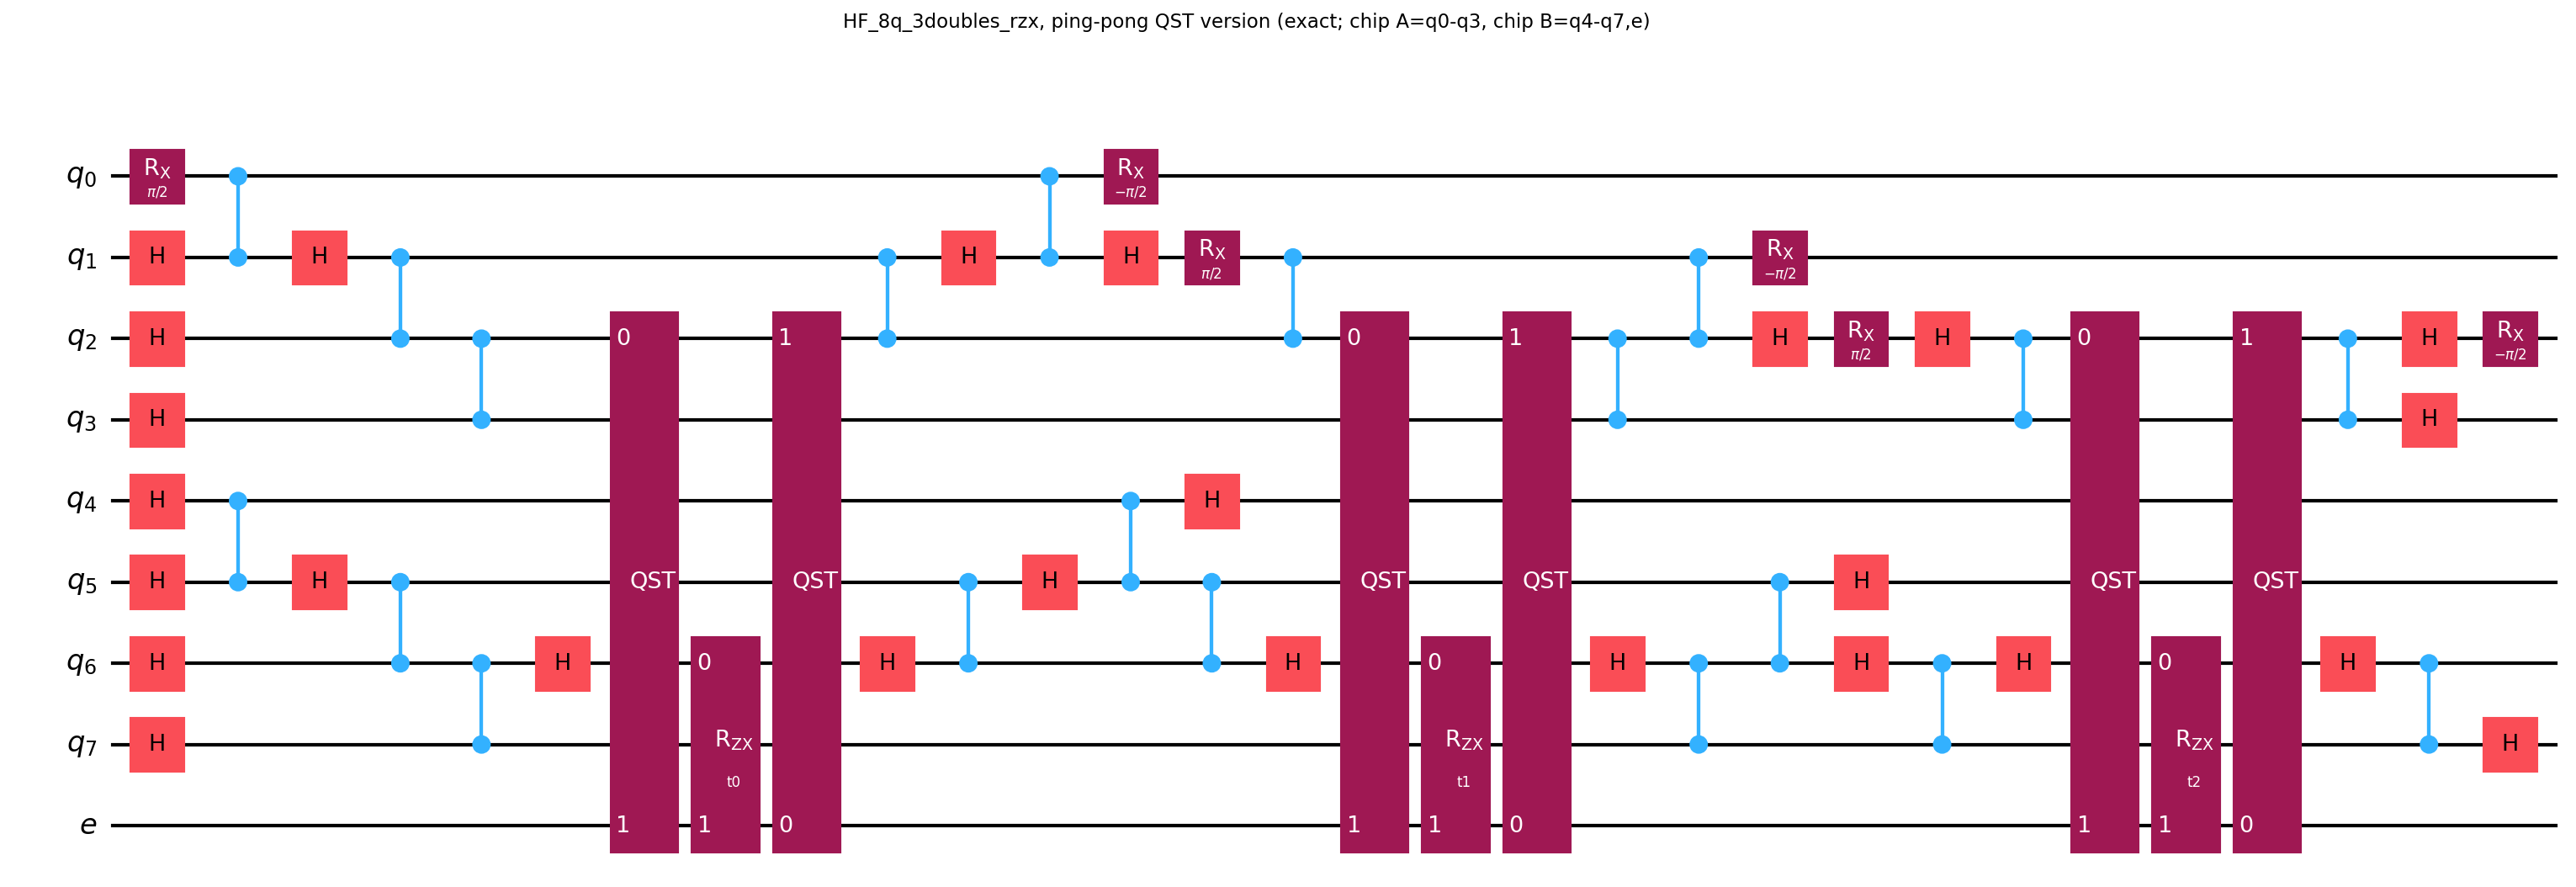
\includegraphics[width=\textwidth]{fig5_HF_pingpong.png}
\caption{\texttt{HF\_8q\_3doubles\_rzx} in ping-pong form: exact, runnable
with the current ansatz. Each crossing is QST out / local $\RZX$ / QST back.}
\label{fig:hfpp}
\end{figure}

\subsection{Why this ansatz cannot migrate}

Between $\RZX(t_0)$ and $\RZX(t_1)$ the circuit applies
$\mathrm{CZ}(q_1, q_2)$ (with gates on $q_1$ in between, so the pair does
not cancel) --- with $q_2$ abroad this is exactly the blocked pattern of
Section~\ref{sec:blocked}. The mirror choice fails identically: $q_6$
participates in $\mathrm{CZ}(q_5, q_6)$ between crossings, and $q_5$ stays
on chip B. The parity ladders of the three doubles re-dress both seam qubits
between every pair of crossings.

\subsection{The desired circuit structure}

Figure~\ref{fig:hfmig} is the \emph{template} a redesigned ansatz must
match: $q_2$ migrates once; between crossings, chip A layers
$V_{A}$ act only on $\{q_0, q_1, q_3\}$ (the $q_2$ wire is empty), while
chip B layers $V_{B}$ may freely dress $q_4\ldots q_7$ and even $e$
(single-qubit gates on the migrated state are allowed); after the last
crossing $q_2$ returns. Total: 2 traversals for all three doubles.

Concretely, the redesign task for the excitation ladders is: route the
fermionic parity of each double onto $q_6$ using \emph{chip-B} CNOT/CZ
ladders, and onto the $\alpha$-sector representative \emph{before} the
migration (or after the return), so that $q_2$'s only two-qubit partners
while abroad are $q_6$/chip-B qubits. Whether the three doubles
$(3,7\,{\to}\,4,0)$, $(3,7\,{\to}\,5,1)$, $(3,7\,{\to}\,6,2)$ admit such an
ordering at chemical accuracy is checkable classically by exact
diagonalization before anything is run.

\begin{figure}[h]
\centering
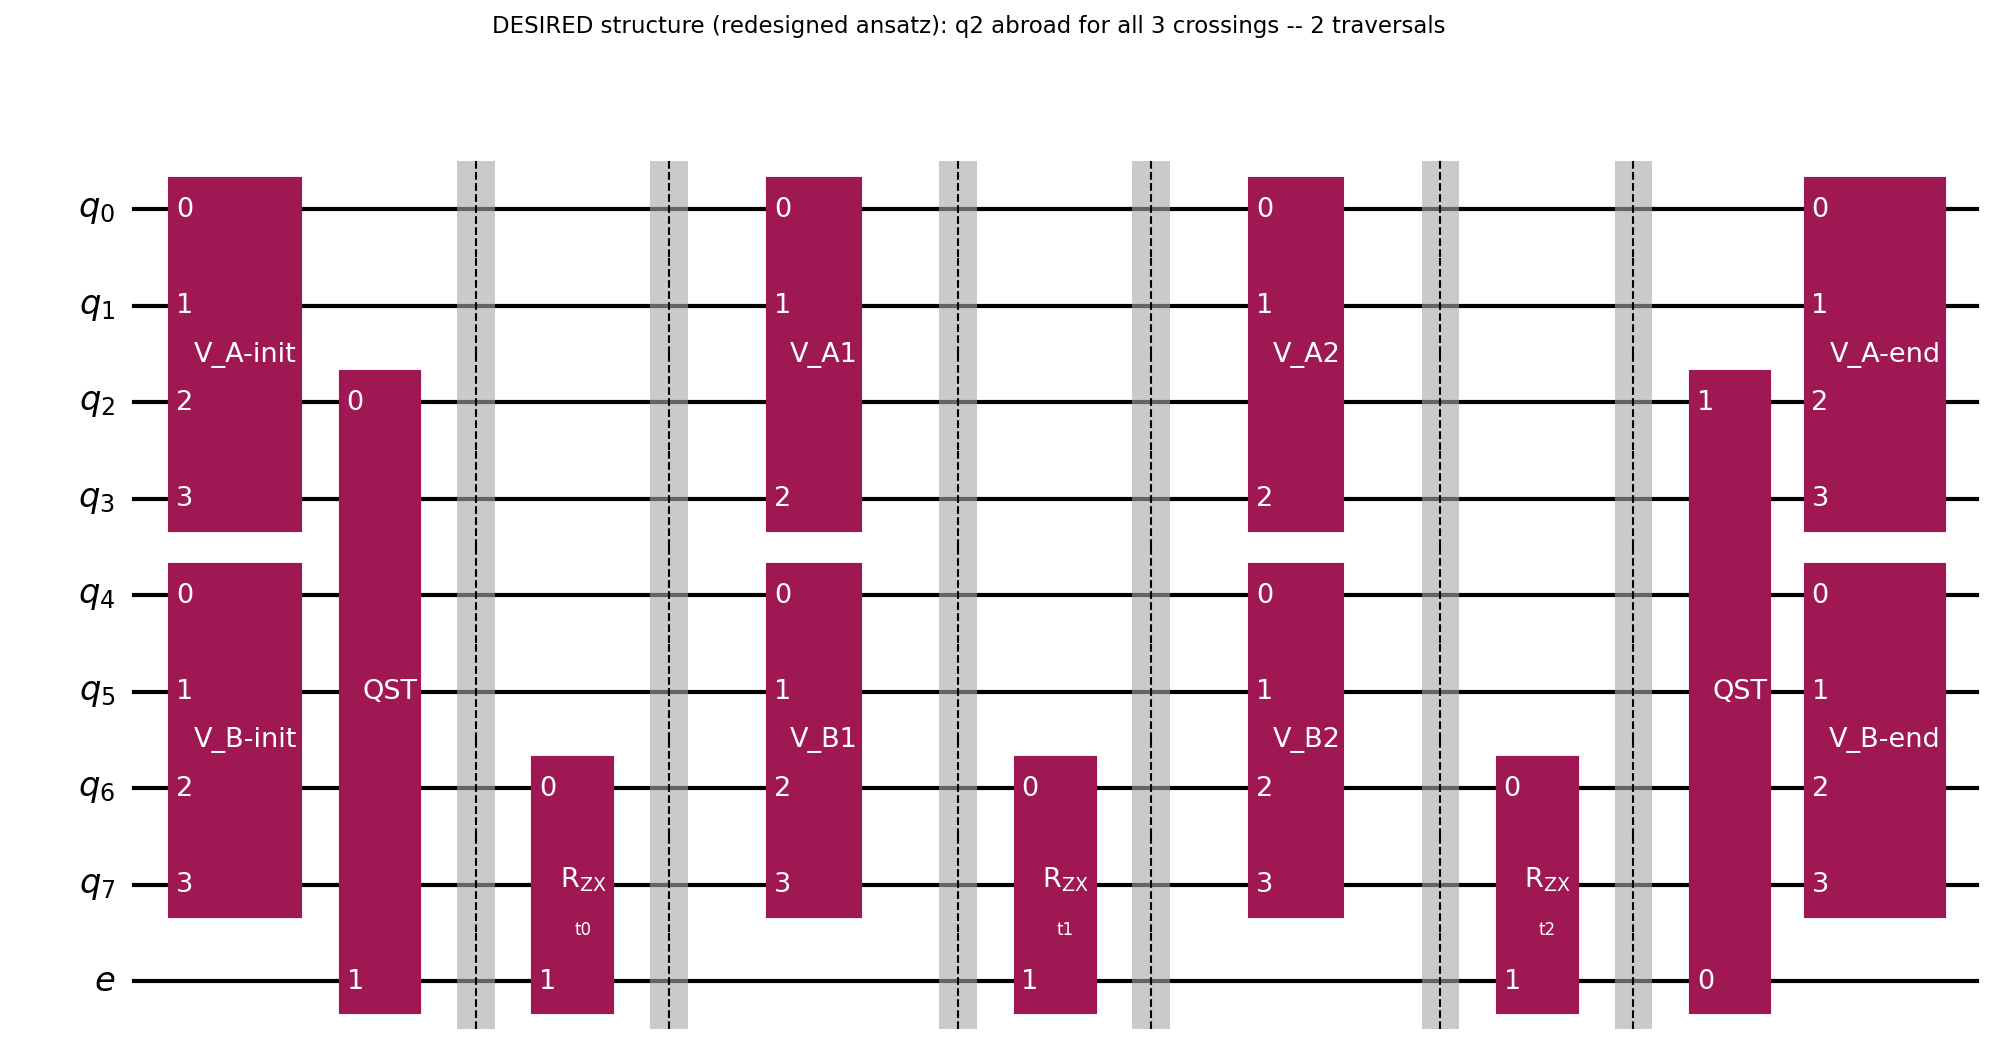
\includegraphics[width=\textwidth]{fig6_HF_migration_template.png}
\caption{Desired structure for a redesigned ansatz (schematic; $V$ boxes are
placeholders): $q_2$ lives on chip B for the whole doubles block, all three
$\RZX(t_k)$ are local, and the cable is used exactly twice.}
\label{fig:hfmig}
\end{figure}

\section{Cost comparison}

Per-use cable noise $p$ (depolarizing), measurement $500{+}200$~ns,
feedback 200~ns, QST 66~ns, local 2q gate 50~ns:

\begin{center}
\begin{tabular}{lccc}
\toprule
Scheme & Cable uses on data & Measurements & Seam time \\
\midrule
Direct $\RZX$ $\times 3$          & 3 (2-qubit exposure) & 0 & ${\sim}150$ ns \\
Ping-pong (Fig.~\ref{fig:hfpp})   & 6 (1-qubit exposure) & 0 & ${\sim}0.5\,\mu s$ \\
Migration (Fig.~\ref{fig:hfmig})  & \textbf{2} (1-qubit exposure) & 0 & ${\sim}0.3\,\mu s$ \\
EJPP telegate $\times 3$          & 0 (ancilla-only)     & 6 & ${\sim}5{-}6\,\mu s$ \\
\bottomrule
\end{tabular}
\end{center}

At equal per-use noise, ping-pong roughly ties the direct gate
($6 \times p/2$ vs $3 \times \tfrac{15}{16}p$ average infidelity) --- its
value is that it wins whenever a passive 66~ns transfer is cleaner than a
full cross-chip entangling gate, and that it needs no measurement hardware.
Migration is a strict $3\times$ improvement over ping-pong and beats the
direct gate at any $p$, but requires the ansatz redesign above. EJPP keeps
data off the cable entirely (and allows heralding/distillation) at the price
of mid-circuit measurement, readout error, and feedforward latency. All
coherent schemes still require the seam-located twirling{+}PEC layer to
reach chemical accuracy at $p \sim 0.1$.

\section*{Reproducibility}

All figures and all unitary-equivalence checks
(\texttt{Operator.equiv} at random parameter bindings) are produced by
\texttt{make\_state\_transfer\_circuits.py} in this folder:
\begin{center}
\texttt{python3 make\_state\_transfer\_circuits.py}
\end{center}

\end{document}
